\documentclass[a4paper, 11pt]{report}

\usepackage{draftwatermark}
\SetWatermarkText{\textbf{PROOF}}
\SetWatermarkScale{1}

\usepackage{geometry}
\geometry{
a4paper,
total={170mm,257mm},
left=20mm,
top=20mm,
}
\setlength\parindent{0pt} % get rid of the stupid indent

% INCLUDE PACKAGES

% \usepackage[utf8]{inputenc}
\usepackage[dvipsnames, table]{xcolor}
\usepackage{float}
\usepackage{graphicx}
\usepackage{tabularx}
\usepackage{fontawesome}
\usepackage[colorlinks=true, linkcolor=Magenta, breaklinks=true]{hyperref}
\usepackage{ragged2e}
\usepackage{cancel} % used to cancel out numbers in maths mode.
\usepackage{amssymb} % gives more maths symbols
\usepackage{enumitem} % gives ability to have different enumerate bullets.
\usepackage{multirow}

\usepackage{longtable}
\usepackage{multirow}

\usepackage{fontspec}
\setmainfont[Ligatures=TeX]{Montserrat}
\setsansfont[Ligatures=TeX]{Montserrat}
\usepackage[raggedright,bf,sf]{titlesec}

% formatting of header/footer and table of contents if the documentclass is an article. This gets ignored if documentclass is article.
\makeatletter
\@ifclassloaded{report}{%
\setcounter{tocdepth}{0}
\renewcommand{\chaptername}{Section}
\renewcommand\chapter{\if@openright\cleardoublepage\else\clearpage\fi
\thispagestyle{fancy}%
\global\@topnum\z@
\@afterindentfalse
\secdef\@chapter\@schapter}
}
\makeatother

% remove hyphenation at end of line
\tolerance=1
\emergencystretch=\maxdimen
\hyphenpenalty=10000
\hbadness=10000

% better table padding
\renewcommand{\arraystretch}{1.6}

% redefine \today to become yyyy-mm-dd format for use in the footer to show export date
\usepackage[yyyymmdd]{datetime}
\renewcommand{\dateseparator}{-}

\usepackage{fancyhdr}
\pagestyle{fancy}
\fancyhf{}
\fancyhead[R]{\leftmark}
\fancyfoot[C]{\thepage}
\renewcommand{\footrulewidth}{0.4pt}
\addtolength{\topmargin}{-1.59999pt} % This and line below changes margins to accomondate for headers and footers
\setlength{\headheight}{13.59999pt}

% NOW CREATE TITLE PAGE

\newcommand{\bookTitle}[4]{
    \begin{titlepage} % Suppresses headers and footers on the title page
	
        \centering % Centre everything on the title page
        
        \rule{\textwidth}{0pt} % Thick horizontal rule
        
        \vspace{0.3\textheight} % Whitespace between the top rules and title
        
        % \rule{\textwidth}{1pt}\\
        \vspace{15pt}
        {\LARGE \textbf{VENTURER CAMP 2023}}\\[1em] % Title line 1
        %{\Large - }\\[0.5\baselineskip] % Title line 2
        {\LARGE #1} \\[15pt]% Title line 3
    
        {\large #2 \\[5em]}
    
        {\large #3} % Date
        \vspace{15pt}
        % \rule{\textwidth}{1pt}
        \vspace{3em}
        %\vfill % Whitespace between the author name and publisher
        
        
        \begin{figure}[H]
            \begin{minipage}{0.45\textwidth}
                \centering
                
\includegraphics[width=0.45\textwidth]{../vc23.png} %this will be replaced with vc23 logo when we have one
            \end{minipage}\hfill
            \begin{minipage}{0.45\textwidth}
                \centering
                \includegraphics[width=0.45\textwidth]{../wcf.png}
            \end{minipage}\hfill
        \end{figure}
    
        \vfill  
        
    \end{titlepage}

    \fancyhead[L]{#1}
    \fancyfoot[L]{\footnotesize{\texttt{#4}\\\texttt{\today}}}
}

\newcommand{\shortTitle}[4]{
        
 
        \begin{figure}[H]
            \begin{minipage}{0.65\textwidth}
                {\LARGE \textbf{VENTURER CAMP 2023}}\\[1em] % Title line 1
                %{\Large - }\\[0.5\baselineskip] % Title line 2
                {\LARGE #1} \\[1em]% Title line 3
            
                {\large #2 \\[1em]}
            
                {\large #3} % Date
            \end{minipage}\hfill
            \begin{minipage}{0.3\textwidth}
                \centering
                
\includegraphics[width=0.9\textwidth]{../vc23.png}
            \end{minipage}\hfill
        \end{figure}

    \fancyhead[L]{#1}
    \fancyfoot[L]{\footnotesize{\texttt{#4}\\\texttt{\today}}}
}

% command for back page of longer documents
\newcommand{\backPage}{
    \begin{titlepage}
        \centering
        \rule{\textwidth}{0pt}
        \vfill
        \begin{figure}[H]
            \begin{minipage}{0.45\textwidth}
                \begin{flushright}
                
\includegraphics[width=0.1\textwidth]{../vc23.png} %this will be replaced with vc23 logo when we have one
                \end{flushright}
            \end{minipage}\hfill
            \begin{minipage}{0.45\textwidth}
                \includegraphics[width=0.1\textwidth]{../wcf.png}
            \end{minipage}\hfill
        \end{figure}
        
        \small{Venturer Camp 2023, a project by \href{https://woodcraft.org.uk}{Woodcraft Folk}, will bring together 13-17 year olds from across the UK to camp together and live by the Woodcraft Folk values for a week in the summer of 2023.\\
        Check out our website (\href{https://venturercamp.org.uk}{venturercamp.org.uk}) and our social media pages for more information.}
        \rule{\textwidth}{2pt}
        \footnotesize{Woodcraft Folk is a registered charity in England \& Wales (1148195) and in Scotland (SC039791), and a limited company, registered in England \& Wales (8133727). Registered office: Holyoake House, Hanover Street, Manchester M60 0AS}
    \end{titlepage}
}




\usepackage{ragged2e}

\newcommand{\nl}{\newline}
\newcommand{\infoemail}{\href{mailto:info@venturercamp.org.uk}{\texttt{info@venturercamp.org.uk}}}

\begin{document}
\bookTitle{Info Pack v2}{subtitle}{23rd June 2023}{info-pack-v2}
\tableofcontents
\chapter{Introduction}
Welcome to info pack v2!\nl

Apologies this info pack is once again slightly later than promised! Many of the team have had exams but we've also been working really hard to make camp as fun and safe as possible. This document should include everything you need to know ahead of the event that we haven't told you already.\nl 

At the time of writing we've got an exciting 409 people booked to attend! If you haven't booked yet and you would like to, this is still possible but at a greater cost and we can unfortunately no longer guarantee we will be able to meet any complex access requirements. More info in our \href{https://venturercamp.org.uk/wp-content/uploads/2023/05/payment-policy-v2.pdf}{payment policy}.\nl

If you've got a question or would like to know some more information, feel free to drop us a DM on our social media or send us an email (\infoemail).

\section{Venturer Camp 2023, a reminder}
Back for 2023, Venturer Camp will once again be returning to Woodcraft Folk's Biblins Youth Campsite in Wye Valley near Hereford from the 5th to 12th August 2023. Venturer Camp is open to participants aged 13-17 inclusive, this due to the Covid pandemic, and will have the theme of Mythology.

\section{Find Out More}
Venturer Camp lives across the internet. You can find out more about us on our website (\href{https://venturercamp.org.uk}{\texttt{venturercamp.org.uk}}), on the Woodcraft website (\href{https://woodcraft.org.uk}{\texttt{woodcraft.org.uk}}), on our Instagram (\href{https://www.instagram.com/venturercamp/}{\texttt{@venturercamp}}) and on our Facebook (\href{https://www.facebook.com/wcfventurercamp}{\texttt{/wcfventurercamp}}).
We will also send emails to those who have booked and to Venturer group contacts with key information in it.

\section{Future Publications}
We are aiming to publish the village handbook by 22nd July 2023. This will contain most of the information which you will need on site including a map, health and safety information, the Code of Conduct and more. This will also be provided to villages on site in print.

\chapter{Communications during the event}
As promised in the last info pack, we will have a WhatsApp number available for you to use during the camp to contact the site. This number is active from now however will not be checked regularly. The number will be checked regularly from 22nd July until after camp.
\begin{table}[H]
    \centering
    \begin{tabular}{p{0.3\textwidth} p{0.6\textwidth}}
        \hline
        Email & info@venturercamp.org.uk\\
        \hline
        WhatsApp & +44 7716 372651\\
        \hline
        Phone & 01600 890 850\\
        \hline
    \end{tabular}
    \caption{Contact methods during the event}
\end{table}

\section{Mobile Phones}
It is up to individual villages to decide appropriate rules for mobile phone usage for participants. This decision should take into account the lack of mobile signal on site and the lack of charging facilities on site.\nl

Villages should consider and make allowances where needed, for those who need their mobile phones as a medical device. There will be charging available in the cabin for those who need their phone for this reason, we would recommend the use of power packs for this. 

\section{Village Coordinator's Meeting}
On site during the event, Village Coordinators will be invited to a morning meeting with Thomas Boxall, camp coordinator, where they will be able to find out the latest information on everything ranging from programme to waste collection. Morning circles within villages shouldn't be held until after the village coordinators meeting to ensure the most up to date information is disseminated to young people. 

\chapter{Getting To Biblins}
The full address of the site is as follows:\\
Biblins Youth Campsite\\
The Doward\\
Whitchurch\\
Ross-on-Wye\\
HR9 6DX\\
OS grid reference: SO 549 145

\section{By Car}
From the A40, Ross-on-Wye to Monmouth road, leave the dual carriageway at Crockers Ash, and follow the signs to Biblins Campsite. Note that access is via a single vehicle width track with passing places, which is unsuitable for coaches or vehicles over 6ft wide.\nl

Special arrangements can be made for coaches to approach from the Gloucestershire side of the river via 3 miles of forestry track. This is a locked route and only available by prior arrangement with us. Your group will then need to carry their luggage over the suspension footbridge.\nl

Please be aware that the lanes close to Biblins Campsite are very narrow, with passing places, and that some Sat Nav systems have directed previous campers along Sandyway Lane, which is NOT suitable for large vehicles.\nl

If you are arriving along the A40 from the north (i.e. from Ross-on-Wye), leave the A40 at the turn for Stoney Hill Industrial Estate; Crockers Ash and Doward. Then turn immediately right and remain on this road for about half a mile - do not turn left into Sandyway Lane (opposite). After half a mile, turn left at the sign to Doward and Biblins (also signed toward Doward Park Campsite). Remain on this road until you reach Doward Park Campsite and then follow the adjacent Forestry Track down the hill to Biblins.\nl

\section{By Public Transport}
From Hereford station - 36 bus towards Over Mannow - takes around 1 hr 15 minutes\nl

From Newport (South Wales) station - Queensway Q6 bus towards Monmouth - takes around 2 hours\nl

From Monmouth walk down the river Wye to the campsite - around 4km - might want someone else to take kit but walk is flat with good views\nl

\subsection{Taxis from Monmouth}
\begin{table}[H]
    \centering
    \begin{tabular}{p{0.3\textwidth} p{0.6\textwidth}}
        \hline
        Amber Cars & 01600 712200\\
        \hline
        Kenny's Taxis & 07828 882432\\
        \hline
    \end{tabular}
    \caption{Taxi firms based near Monmouth}
\end{table}

\subsection{Shuttle Busses}
There will be shuttle buses running from Hereford station on the first day of camp and back to Hereford station on the last day of camp. Please get in touch with \href{mailto:coaches@venturercamp.org.uk}{\texttt{coaches@venturercamp.org.uk}} if you haven't already if you require a shuttle bus or have any questions. 

\chapter{Equipment}
\section{Kit List}
Anything brought to camp is brought at the owners risk. We recommend not bringing valuables or keeping them on your person at all times.
\subsection{It is suggested that everyone on site brings}
\begin{itemize}
    \item Sleeping bag
    \item Pillow, roll-mats etc
    \item Eating Kit
    \item Wash Kit
    \item Any medications that are needed
    \item Any menstrual products that may be needed
    \item Clothes (be prepared for all weathers)
    \item Torch
    \item Waterproof jacket \& trousers (if you have them)
    \item Boots/ outdoor shoes which are comfortable to hike in
    \item Flip-Flops/ sandals
    \item Towel
    \item Something to put dirty laundry in
    \item A refillable water bottle
    \item Sun Cream
    \item Hat
\end{itemize}
There will also be an opportunity to purchase merchandise and additional food \& drinks on site. Pricing information will be made available in info pack v2.  
\subsection{Participants wishing to take part in the Adventurous Activities will also need}
\begin{itemize}
    \item Clothes you don't mind getting wet \& dirty in the river
    \item Spare bin bag for wet clothes
    \item Towel you don't mind using straight out of the river
    \item Snug fitting trainers
\end{itemize}
\subsection{Do not bring}
Anyone found on site with the items listed below may have the item confiscated
\begin{itemize}
    \item Nuts or products containing nuts
    \item Hi-vis jackets
    \item Walkie Talkies/ handheld radio communication devices
    \item National Flags
    \item Hair Straighteners/ Dryers
    \item Unnecessary Electrical items
    \item Items of high sentimental/ monetary value.
\end{itemize}

\section{Equipment On Site}
Nobody is to take any equipment from any store cupboards on site without consulting with the Site Services team. The Site Services team will be more than happy to support with finding equipment/ materials if needed.

\section{Broken Equipment at The End of Camp}
Things break, we definitely learnt this at Common Ground! If something breaks, please don't leave it on site for us to clear up - Biblins has limited waste disposal which we will already be pushing to its limits from the numbers of people on site so adding broken tents, air mattresses or other equipment to this will make the job really tough for the site services team \& staff team at Biblins.\nl

If you need support breaking down broken equipment to be able to fit it back in your van, contact Site Services.

\chapter{Site Layout}
There are some areas of the site which we are still to finalise, these will be finalised in the coming weeks and confirmed either via social media or through the village handbook. 
\begin{figure}[H]
    \centering
    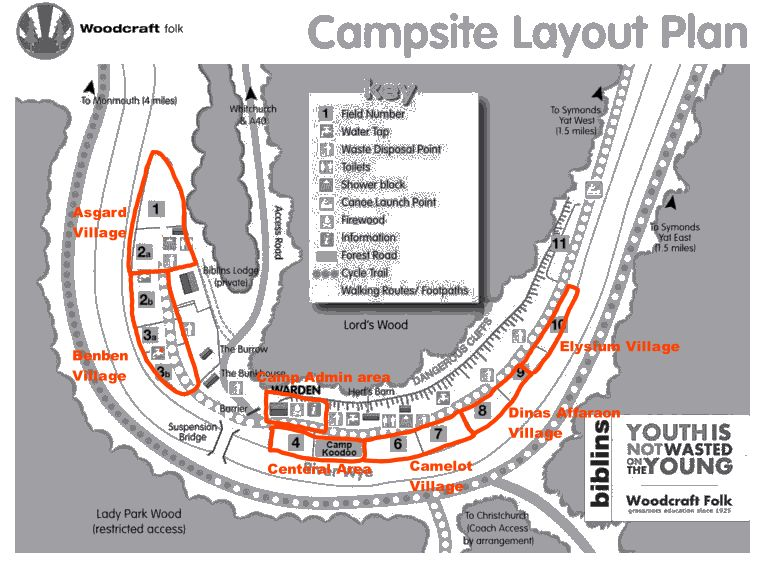
\includegraphics[width=0.9\textwidth]{camp-map-v1.jpg}
    \caption{Camp Outline Map}
\end{figure}
Not shown in the map above:
\begin{itemize}
    \item Camp Koodoo has moved to above pitch 1, this means where camp Koodoo is marked on the map will be pitch 5 which will form part of our central area,
    \item part of pitch 4 will be used as the ``Site Yard'' and will be home to the food distribution centre as well as the site services depot and car park, and
    \item pitch 11 will be used as canoe storage and the launch site for them. 
\end{itemize}

There will be a much nicer version of the map made before camp, don't worry!

\chapter{Villages}
The campers at Venturer Camp 2023 will be split between five villages.
\section{Names of Villages}
The five Villages at Venturer Camp are named for mythical, magical places from ancient traditions and beliefs
\begin{description}
    \item[Asgard] is one of the Nine Worlds in ancient Norse mythology, and is the fortress home of the most powerful gods, including Odin and Thor. It is also the location of Valhalla, the mighty hall that is home to the souls of warriors killed in battle. The realm of Asgard is connected to the mortal world, Midgard, by a rainbow bridge.
    \item[Benben] is the first mound of land that rose up out of the primordial waters when the world was first created, according to ancient Egyptian religious belief. The creator-god Atum settled on the mound before creating the air-god Shu and water-goddess Tefnut, who made the sky and the earth.
    \item[Camelot] is home to King Arthur's court. It is a silly place.
    \item[Dinas Affaraon] in Welsh tradition, was home to the Pheryllt, a tribe of Druids skilled in alchemy. It was a fortified hill city, known also as the 'hill of higher powers'. It is also mentioned in one of the mediaeval legends that make up the Mabinogion as the place where King Ludd imprisons the white Saxon dragon and the red dragon of Wales, locked in eternal battle.
    \item[Elysium] was the ancient Greek afterlife, a paradise located in the ocean at the western end of the earth, and was ruled over by the Titan, Kronos, the father of Zeus. Elysium, where those favoured by the gods live on after death, is also known as the Isle of the Blessed - in its fields it is always spring.
\end{description}

\section{Coordination Team's Village Placement}
Each village will contain a few of the central coordination team as we don't have the resources to support a `Central Village'.\nl

The central team may need slight accommodations made within the village for them, for example, meals being kept back for them to eat at different times, no village roles being assigned, or being exempt from clan. Support with supporting the central team to also have a good experience at Venturer Camp 2023 is available from the Coordination \& Event Administration team (\infoemail).\nl

A list of those who are in each village and designated as central team and may need accommodations made will be made available in the village handbook. The number of central team in each village has been carefully considered and is as equal as possible between the different villages.

\section{Village Equipment}
A few Woodcraft Folk districts and Biblins are very kindly lending us their kit to support villages, so all you need is personal kit (sleeping tent, sleeping bag, eating kit etc). However you will need to help put this up and take it down as a village, and take care of it!\nl

We are still finalising the village equipment and will have this confirmed before June 30th. 

\section{Village Composition}
\subsection{Asgard - pitches 1a, 1b \& 2a}
\begin{itemize}
    \item Newham Watersmeet
    \item Cambridge
    \item St Albans
    \item Eastern Region
    \item Sheffield Derwent
    \item Sheffield Porter \& Don
    \item Birkenhead
\end{itemize}
\subsection{Benben - pitches 2b, 3a \& 3b}
\begin{itemize}
    \item Clapham
    \item Highgate \& Holloway
    \item Teddington
    \item New Barnet
    \item Camps For All
    \item Banbury
    \item Stroud
    \item Food Team
    \item Woodcraft Folk Staff
    \item International Volunteers
\end{itemize}
\subsection{Camelot - pitches 6 and 7}
\begin{itemize}
    \item Lewisham \& Greenwich
    \item Exeter
    \item Brighton \& Hove Central
    \item Watford
    \item Eastbourne
    \item Tyne
    \item Leeds
    \item Coach Coordinators
    \item Camp Coordinators
\end{itemize}
\subsection{Dinas Affaraon - pitches 7 - 9}
\begin{itemize}
    \item Oxford
    \item Hackney
    \item Brighthelmstone
    \item Bath
    \item MEST-UP Centre Team
    \item Adult Volunteers
\end{itemize}
\subsection{Elysium - pitches 9 \& 10}
\begin{itemize}
    \item Scotland
    \item Machynlleth
    \item Cardiff
    \item Manchester
    \item Southampton
    \item Ealing
    \item Bromley
\end{itemize}

\section{Village Roles}
Each village will need to identify individuals (or teams, we would recommend every role nominates a Deputy) to take on the following roles:
\begin{itemize}
    \item Village Coordinator
    \item KP (this works really well as a team, food will be provided centrally but each village needs someone to oversee the cooking!)
    \item Safeguarding Lead
    \item Deputy Safeguarding Lead
    \item First Aid Lead
\end{itemize}
There may be some additional roles asked for in the future, however the five above are our priority.\nl

Please ensure \href{https://forms.gle/HrV2H4Yyr1tsCpBGA}{this form} is completed by all post holders in your village by 30 June so each role holder can be sent information relevant to their role and keeping everyone safe at Venturer Camp - if you are struggling to fill roles or have any questions please get in touch with the Venturer Camp team. 

\section{Clans}
The daily timetable (\textit{Table \ref*{tab:daily-timetable}}) has been laid out in a way that means most volunteers can do clan, especially in the morning. However some central volunteers may need to miss clan due to other responsibilities. We would recommend that you discuss their availability with them and spread them out when you create your clan groups. \nl

Every village will be expected, at a minimum, to have the following clans
\begin{itemize}
    \item Cooking
    \item Washing Up
    \item Site Services Support (cleaning toilets in the morning and evening, litter pick in the afternoons)   
\end{itemize}
Villages may also choose to put clans in charge of wood and water, programme, or anything else they wish. 


\chapter{Programme}
\section{Daily Timetable}
\begin{table}[H]
    \label{tab:daily-timetable}
    \centering
    \begin{tabular}{p{0.2\textwidth} p{0.2\textwidth} p{0.5\textwidth}}
        \textbf{Start} & \textbf{End} & \textbf{Content}\\
        \hline
         & 1430 & Village Mornings (this will include rotating adventurous activities \& lunch) \\
        \hline
        1430 & 1600 & Central Programme slot 1 \\
        \hline
        1600 & 1630 & Break \\
        \hline
        1630 & 1730 & Central Programme slot 2 \\
        \hline
        1730 & 1800 & Break \\
        \hline
        1800 & 1930 & Dinner \\
        \hline
        1930 & 2030 & News \\
        \hline
        2030 & 2200 & Evening Programme slot 1 \\
        \hline
        2200 & 2230 & Sign In \\
        \hline
        2230 & 2330 (or 0100 on 11/08/23) & Evening Programme slot 2 \\
        \hline
    \end{tabular}
    \caption{Daily Timetable}
\end{table}
The daily timetable will be confirmed in the village handbook with further information about which centres are offering workshops when as well as when different villages will be able to take part in the adventurous activities. 

\section{Mini-Themes}
There will be 3 different mini themes on camp, as part of the wider theme of mythology. Every two days there will be a different mini theme working towards the central programme night, where this will be the dress up theme. There will also be some relevant workshops, and the Wide Game will fit into this too.

\begin{table}[H]
    \centering
    {\RaggedRight
    \begin{tabular}{p{0.3\textwidth} p{0.6\textwidth}}
        \textbf{Dates} & \textbf{Theme}\\
        \hline
        6th - 7th August & European mythology (Celtic, Norse etc)\\
        \hline
        8th - 9th August & Ancient mythology (Greek, Roman, Egyptian etc)\\
        \hline
        10th - 11th August & Mythology from around the world (essentially anything that doesn't fit into the above!)\\
        \hline
    \end{tabular}
    }% end of \RaggedRight
    \caption{Mini-Theme breakdown by date}
\end{table}
The first night is also a big programme night, and the dress up theme for this will just be mythology in general. \nl

We recommend you discuss cultural appropriation in your group ahead of camp to ensure no one plans a costume that could be culturally offensive.

\section{Centre Activities}
\subsubsection{Sign Up}
We will give sign up sheets to village coordinators each morning in the village coordinator meeting at 08:30am. Sign up for workshops in centres will take place in villages each day for workshops that day, until 02:00pm when we will collect the sheets and put them outside the relevant centres. There will be limited spaces for each workshop per village to ensure the workshops are safe and enjoyable. If there are any spaces left for workshops these will be available on a first come first serve basis once activities start at 02:30pm.

\subsection{Centres}
\begin{description}
    \item[Activism] a space full of activities about the climate, anti-racism, LGBTQI+ rights, feminism and more. This centre aims to encourage people to challenge the 'black and white, good or bad' view often found in activist circles and communities and instead explore issues from a more holistic point of view. There will be lots of exciting special guests running workshops as well as our excellent volunteers.
    \item[Arts] a tent to explore and practise all kinds of art: visual, performance, couture, classic and modern. At drop in time it will be a calm space for venturers to chill out and sit with their own crafts. Workshops will mostly be a bit more active with a different disciplinary focus each time. The centre will become a gallery of itself as camp goes on.
    \item[Mythology] a centre to explore the camp theme of mythology through lots of  different kinds of activities, from craft to games to discussions.
    \item[Media] a space where you can be guided through the process of drafting, filming and editing together videos. These will be watched by everyone on camp in the main marquee, as part of the News each night.
    \item[Solar Cinema] a centre where you can see blockbusters and smaller releases, including some bigger events where discussions and Q\&A sessions follow the film. Some viewings may be outside of typical centre hours, but we will make timings clear in the programme attendees are given on site.
    \item[Radio] a centre where Venturers can run their own radio programme, be that a talk show, an interview, simply djing, or a mixture. There will be regular radio programmes throughout camp, so you should bring an FM radio from home if you have one (we will provide some to villages and centres but more would be good)!
\end{description}

Planning is ongoing for some bushcraft activities and MEST-UP provision (peer support and resources on topics such as relationships and intoxicating substances), but these centres are not yet confirmed and may be open just for limited drop in or at specific advertised activity times rather than the whole time other centres are open.

\chapter{Safeguarding \& Risk Management}
\section{Safeguarding Team}
Safeguarding support and response will be provided by an on-site Safeguarding Team, which includes:
\begin{itemize}
    \item Debs McCahon
    \item Felix Pepler
    \item Catherine Tuffrey
\end{itemize}
Each Village will be also required to nominate a Safeguarding Lead.

\section{Site Stewards}
Volunteer stewards will also be available on site - stewards will be available at the Information Desk immediately outside the Biblins Cabin. Stewards will take responsibility for:
\begin{itemize}
    \item Signing people on and off site
    \item Directing cars and deliveries
    \item Answering questions
    \item Signposting campers to team members
    \item First point of contact for any concerns
\end{itemize}

\section{DBS/ PVG Screening}
All campers aged 18 years and over will need to follow Woodcraft Folk's \href{https://woodcraft.org.uk/resources/volunteer-screening/}{Screening \& Vetting procedures}, this includes: 
\begin{itemize}
    \item Submitting two suitability references
    \item Completing an enhanced DBS 
    \item PVG membership (in Scotland only) 
\end{itemize}

Time is running out if you need to apply or update your DBS. Please contact your District Membership Secretary or \href{mailto:membership@woodcraft.org.uk}{\texttt{membership@woodcraft.org.uk}} for help with your DBS or PVG application. Any individual without a current DBS before 31st July will be asked not to attend and alternative adult support will need to be identified.

\section{Responding to incidents, accidents and disclosures}
If you would like to discuss any safeguarding or child protection issues please contact \href{mailto:safeguarding@woodcraft.org.uk}{\texttt{safeguarding@woodcraft.org.uk}}.

\section{First Aid}
Each village is expected to ensure they have access to a competent First Aider. In the Biblins environment this should be an individual who has a current First Aid qualification. For more information about Woodcraft Folk's expectations please see \href{https://woodcraft.org.uk/resources/first-aid-guidance/}{the first aid guidance on the Woodcraft Folk website}.

\chapter{Site Safety}
Group leaders are reminded that they are responsible for the safety and well-being of the young people in their group at all times. Please see Woodcraft Folk's latest residential \href{https://woodcraft.org.uk/group-guidance/camping-and-residentials/}{guidance on the Woodcraft Folk Website}. \nl

There are some aspects of the site which Group leaders should be aware of including:
\section{Public Access}
There are a number of rights of way through the site, including access to the bridge in the centre of the campsite, which are well used by walkers. Thought should be given to the positioning of tents, marquees and cars to create natural barriers to the camping circle. Anyone in the camping circle without a Venturer Camp wristband should be politely challenged and asked to return to the public footpath.

\section{The River Wye}
Many of our camping pitches back directly onto the river, while the riverbank is clearly marked, it is not fenced. \nl

The river is fast moving and not suitable for swimming in. Canoes may launch from the launch on the eastern end of the site. Access to the river from anywhere else along the river bank is not permitted. 

\section{Vehicles on Site}
Groups are asked to keep driving on site to the absolute minimum needed to arrive/leave site with their group.  There is a speed limit of 10 miles per hour and drivers should be aware that the path through the site is very popular with local walkers as well as being used by other campers.\nl

Vehicles must be parked in the designated car park and not adjacent to villages during the event, unless expressly agreed in advance, e.g. for disabled access.

\chapter{Payments on Site}
Due to the lack of mobile signal and WiFi on site, and the aim to reduce cash use on site, Venturer Camp 2023 will see the return of an on-camp currency.
This currency will be available to be exchanged from GBP during the event and exchanges back to GBP will be available at the end. There may be limited hours during which the camp Bureau de Change will be open, possibly 2-3pm daily. The exchange rate between the on camp currency and GBP will be 1:1.

The on camp currency will be able to be used in the cafe and the shop to purchase refreshments and merchandise. An approximate price list is available below.

\begin{table}[H]
    \centering
    {\RaggedRight
    \begin{tabular}{p{0.5\textwidth}p{0.3\textwidth}}
        \textbf{Product} & \textbf{Price}\\
        \hline
        Pot coffee & 0.50\\
        Nice coffee & 1.00\\
        Nice decaf coffee & 1.00\\
        Iced coffee & 1.50\\
        \hline
        Tea & 0.50\\
        Herbal Tea & 1.00\\
        \hline
        Fruit Smoothie & 2.50\\
        Hot Chocolate & 1.50\\
        \hline
        Dragon Breath Cookies & 0.50\\
        Frost Bites & 0.50\\
        Sea Biscuits & 0.50\\
        \hline
        Cake of the day & 1.00\\
        Cake of yesterday & 0.50\\
        \hline
        Toasties & 1.00\\
        Fabled Oats & 1.50\\
        \hline
    \end{tabular}
    }% end of \RaggedRight
    \caption{Approximate Cafe price list}
\end{table}
The cafe might also offer better value deals - watch this space!
\begin{table}[H]
    \centering
    {\RaggedRight
    \begin{tabular}{p{0.5\textwidth}p{0.3\textwidth}}
        \textbf{Product} & \textbf{Price}\\
        \hline
        Camp t-shirt & 15.00\\
        \hline
        Stickers (2 pack) & 0.50\\
        Sew-on-badge & 1.50\\
        \hline
        Cafe mug & 6.00\\
        \hline
    \end{tabular}
    }% end of \RaggedRight
    \caption{Approximate Merchandise price list}
\end{table}

\chapter{Get Involved}
We are always looking for more people to join the team!\nl

Current roles we are looking to fill:
\begin{itemize}
    \item Centre Coordinator
    \item Stewards
    \item Food Logistics Assistant
    \item Allergy Kitchen Assistant
    \item Cafe Assistant
    \item HACCP Coordinator
    \item Off Site Food Driver
\end{itemize}
If you like the look of a role above and want more information, drop us an email to \infoemail. \nl

If you want to get involved and don't see something listed above which suits you drop us an email to \infoemail. 

\backPage
\end{document}